\chapter{Τεχνικές Προβλέψης Χρονοσειρών}
\label{chap3}

\section{Εισαγωγή}
Μέσα από την εφαρμογή των κλασικών μεθόδων προβλέψεων αποσκοπούμε με χρήση των παρελθοντικών παρατηρήσεων μιας χρονοσειράς να εκτιμήσουμε τις μελλοντικές.
Η πρόβλεψη αποτελεί μια πολυβηματική διαδικασία που θα αναπτυχθεί στο παρόν κεφάλαιο και περιγράφεται από το διάγραμμα ροής του Σχήματος \ref{classicmethodology}.

\begin{figure}[t!]
  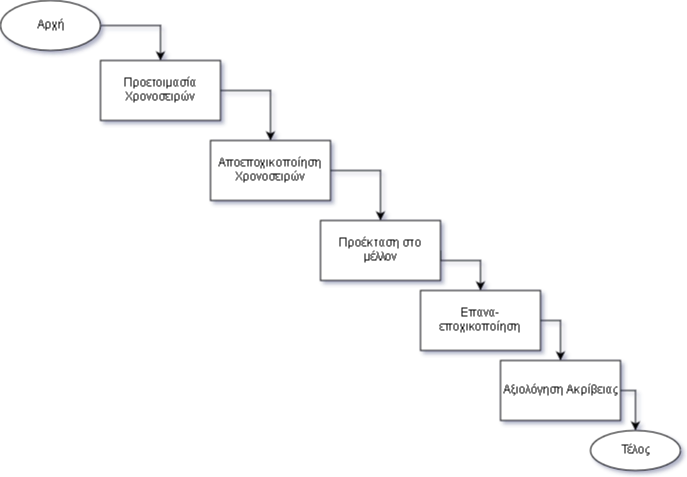
\includegraphics[scale=0.5]{figures/classicforecasting(1).png}
\centering
\caption{Κλασική μεθοδολογία πρόβλεψης χρονοσειρών}
\label{classicmethodology}
\end{figure} 



\section{Προετοιμασία Χρονοσειρών}

\subsection{Γραφική Αναπαράσταση Δεδομένων}
Κατά τη διαδικασία της επεξεργασίας και πρόβλεψης μιας χρονοσειράς είναι σημαντικό ο ερευνητής να μπορεί να αποκτήσει μία διαίσθηση πάνω στα δεδομένα. Μέσω της αναπαράστασης τους σε μια γραφική απεικόνιση μπορεί εύκολα να διαπιστώσει ποια ποιοτικά χαρακτηριστικά της χρονοσειράς έχουν έντονο βάρος. Μπορεί έτσι να εντοπίσει ότι η χρονοσειράς χαρακτηρίζεται από ακραίες τιμές, έχει έντονη τάση ή μοτίβα που επαναλαμβάνονται και εποχιακότητα.



\subsection{Διαχείριση Ιδιομορφίας Χρονοσειρών}
Είναι αρκετά σύνηθες τα δεδομένα που προορίζονται για πρόβλεψη να παρουσιάζουν δυσμορφίες. Μη σταθερή συχνότητα μεταξύ δύο συνεχόμενων τιμών μιας χρονοσειράς τη καθιστά αταίριαστη για πολλές από τις κλασικές μεθόδους πρόβλεψης. Τα δεδομένα βρίσκονται σε συχνότητα διαφορετική από αυτή που θέλουμε να προβλέψουμε, λόγου χάρη ημερήσια, ενώ είναι επιθυμητό να παραχθούν μηνιαίες προβλέψεις.
Επίσης, υπάρχει η περίπτωση ενώ εν γένει η σειρά αποτελείται από τιμές που ισαπέχουν μεταξύ τους στο πεδίο του χρόνου, παρουσιάζονται περιπτώσεις που δεν έχουν σημειωθεί κάποιες παρατηρήσεις. Αυτές τις ελλείψεις τις λέμε κενές τιμές. Μία άλλη ιδιομορφία που μπορεί να συναντήσουμε και καθιστά τη χρονοσειρά μη διαχειρίσιμη από αρκετές μεθόδους είναι η ύπαρξη μηδενικών τιμών. 

\subsubsection{Επαναδειγματοληψία}
Στη περίπτωση που το χρονικό διάστημα μεταξύ δύο παρατηρήσεων δεν είναι σταθερό ή ακόμα και διαφορετικό από αυτό που θέλουμε να έχουμε στη πρόβλεψή μας, πρέπει να φέρουμε τα δεδομένα μας σε μια πιο κανονικοποιημένη μορφή. Μία μέθοδος που μπορούμε να ακολουθήσουμε είναι η μέθοδος της επαναδειγματοληψίας (\en{resampling}). Η χρονοσειρά, συχνά, περιγράφει φαινόμενα συνεχούς χρόνου μέσα από διακριτό χρόνο. Με την επαναδειγματοληψία χρησιμοποιούμε τη πληροφορία που έχουμε ήδη στη διάθεση μας για να δημιουργήσουμε μια νέα χρονοσειρά που της έχουμε ορίσει τους ακριβείς χρόνους των παρατηρήσεων. Η επιλογή αυτή γίνεται τόσο βάσει των τιμών που ήδη έχουμε αλλά και του στόχου μας για το αποτέλεσμα στη πρόβλεψη.

Έχοντας επιλέξει τη νέα συχνότητα των δεδομένων, μένει να επιλέξουμε με ποιόν τρόπο θα γίνει η μετατροπή. Μπορούμε να διακρίνουμε δύο βασικές περιπτώσεις ανάλογα με το αν μεταβαίνουμε από μεγαλύτερη σε μικρότερη συχνότητα. Την δειγματοληψία προς τα πάνω \en{(upsampling)} και τη δειγματοληψία προς τα κάτω \en{(downsampling)}.

Για παράδειγμα, μπορούμε να έχουμε δεδομένα που έχουν συλλεχθεί σε ωριαία βάση, ενώ η πρόβλεψή μας θέλουμε να γίνει σε ημερήσιο επίπεδο. Τότε χρησιμοποιούμε \en{downsampling}, μετατρέποντας τα δεδομένα με μια κατάλληλη συνάρτηση, όπως το άθροισμα των ωριαίων τιμών, ο μέσος όρος τους, το μέγιστο ή το ελάχιστο. Αντίστοιχα αν τα δεδομένα μας θέλουμε να αλλάξουν από μικρότερη συχνότητα σε μεγαλύτερη, όπως από ημερήσια σε ωριαία, χρησιμοποιούμε \en{upsampling}, που συνδυάζεται συνήθως συμπληρώνοντας παρεμβολικά τις νέες χρονικές στιγμές που προκύπτουν. Η παρεμβολή θα περιγραφεί στη διαχείριση κενών τιμών

\subsubsection{Διαχείριση κενών τιμών}
Αρχικά, εφόσον αυτό είναι δυνατό, προσπαθούμε να βρούμε τις τιμές που μας λείπουν από άλλες πηγές, πέραν της αρχικής που λάβαμε τα δεδομένα. Επίσης, αν οι σειρές που αναλύουμε είναι λίγες στο πλήθος και γνωρίζουμε τη φύση της, μπορούμε να ορίσουμε απευθείας τις κενές τιμές, στη περίπτωση που βάσει των παραπάνω μπορούμε να κάνουμε μία ασφαλή εκτίμηση.

Στη πράξη τα παραπάνω δεν είναι συχνά εφικτά, ιδίως στις περιπτώσεις που πρέπει να γίνει διαχείριση μεγάλου αριθμού χρονοσειρών. Έτσι διακρίνουμε δύο περιπτώσεις: χρονοσειρές με εποχιακή συμπεριφορά και μη.

Όταν η χρονοσειρά προς επεξεργασία παρουσιάζει σαφή εποχιακή συμπεριφορά, μπορούμε να εκτιμήσουμε τη τιμή βάσει των τιμών των αντίστοιχων περιόδων με την εν λόγω κενή τιμή. Ένας τρόπος είναι να πάρουμε τον μέσο όρο. Έτσι, αν σε μία ετήσια χρονοσειρά με μηνιαία δεδομένα, αν μας λείπει η τιμή από κάποιον Ιανουάριο, μπορούμε να τη συμπληρώσουμε ως τον μέσο όρο των άλλων.

Στη περίπτωση που δε μιλάμε για εποχιακή συμπεριφορά, χρησιμοποιούμε τη μέθοδο της παρεμβολής για να συμπληρώσουμε τις κενές τιμές μας. Χρησιμοποιώντας τις γειτονικές τιμές μιας ακολουθίας κενών τιμών, τις συμπληρώνουμε με χρήση κατάλληλης μεθόδου. Μια κλασική προσέγγιση είναι να συμπληρωθούν γραμμικά, ως σημεία της ευθείας που ορίζουν οι δύο οριακές τιμές. Ειδάλλως μπορούμε να χρησιμοποιήσουμε άλλες μεθόδους όπως να δώσουμε τη τιμή της πιο κοντινής από τις δύο τιμές, να τις συμπληρώσουμε ως σημεία ενός πολυωνύμου δευτέρου, τρίτου ή μεγαλύτερου βαθμού. Πιο σύνθετες μέθοδοι είναι αυτές των \en{splines, krogh,} βαρυκεντρίκή και πολυωνυμική κατά σημείο.

\subsubsection{Διαχείριση μηδενικών τιμών}
Διακρίνουμε δύο περιπτώσεις, αν η παρατήρηση είναι πράγματι μηδενική ή έχει πάρει αυτή τη τιμή λόγω λάθους στη συλλογή δεδομένων. Προφανώς, στη δεύτερη περίπτωση χειριζόμαστε αυτές τιμές σαν να ήταν κενές και ακολουθούμε τις διαδικασίες που περιγράφηκαν προηγουμένως.

Αλλιώς, αν οι μηδενικές τιμές είναι λίγες, δεν θα επηρεάσουν σε μεγάλο βαθμό τα μοντέλα πρόβλεψης μας. Σε αντίθετη περίπτωση, χρησιμοποιούμε ειδικά μοντέλα για τη διαχείριση διακοπτόμενης ζήτησης.  

\subsection{Ημερολογιακές προσαρμογές}

Η χρονοσειρές είναι συχνό να περιγράφουν τιμές που σχετίζονται με ανθρώπινες ενέργειες και επηρεάζονται από τον τρόπο που είναι οργανωμένη η ανθρώπινη κοινωνία. Έτσι προετοιμάζοντας μια χρονοσειρά για πρόβλεψη πρέπει να εντοπίσουμε με πιο τρόπο συμβαίνει αυτή η επιρροή.

Σε ημερήσιες χρονοσειρές, αυτό γίνεται προσαρμόζοντας τα δεδομένα βάσει ημερολογιακών γεγονότων. Καθορίζουμε, λοιπόν, τις εργάσιμες μέρες συσχετισμένες με το μέγεθος που περιγράφει η σειρά και τις αντίστοιχες αργίες. Έχοντας προσδιορίσει τα παραπάνω, υπολογίζουμε τις εργάσιμες μέρες για κάθε περίοδο των δεδομένων μας ($N_t$) και τον μέσο όρο τους για όλες τις περιόδους ($N_{avg}$).

Μπορούμε έτσι να εξομαλύνουμε τη τιμή της κάθε παρατήρησης μας ως εξής:
\[ Y_t^{'} = Y_t . \frac{N_{avg}}{N_t} \]

\section{Προέκταση χρονοσειρών}

\subsection{Εισαγωγή}

Αφότου έχουμε προετοιμάσει τη χρονοσειρά και την έχουμε αποσυνθέσει στα επιμέρους της στοιχεία, όπως περιγράφηκε στο προηγούμενο κεφάλαιο, προχωράμε στην εφαρμογή κάποιου μοντέλου πρόβλεψης στα αποεποχικοποιημένα δεδομένα. Στόχος στην εφαρμογή του μοντέλου είναι το αποτέλεσμα που θα προκύψει να είναι όσο πιο ακριβές δύναται, δηλαδή οι τιμές που θα παράξει το μοντέλο να είναι όσο το δυνατόν πιο κοντά στις πραγματικές που θα έχουμε στη διάθεση μας με τη πάροδο του χρόνου. Στο παρόν κεφάλαιο θα μελετήσουμε τις στατιστικές μεθόδους πρόβλεψης.

\subsection{\en{Naive:} η αφελής μέθοδος}

H \en{Naive} είναι η πιο απλή μέθοδος στατιστικής πρόβλεψης. Θεωρεί ότι η τιμή που θα ακολουθήσει χρονικά ταυτίζεται με τη τιμή της παρούσας περιόδου, σύμφωνα με τη παρακάτω σχέση, όπου το $F_t$ είναι η πρόβλεψη κατά τη χρονική στιγμή $t$ και $Y_t$ η πραγματική τιμή της σειράς:
\[ F(t+1) = Y(t) \]

Είναι φυσικό ότι η \en{Naive} δεν παράγει ακριβείς προβλέψεις αλλά μπορούμε να τη χρησιμοποιήσουμε ως βάση σύγκρισης (\en{benchmark}) άλλων μεθόδων.

\subsection{Μοντέλα Παλινδρόμησης}

Η ανάλυση της παλινδρόμησης αποσκοπεί στην εύρεση συσχετίσεων μεταξύ μιας εξαρτημένης μεταβλητής και μίας ή περισσοτέρων ανεξάρτητων μεταβλητών. Έχει ευρεία χρήση στη διαδικασία των προβλέψεων, τόσο ως μοντέλο πρόβλεψης αλλά και ως υποβοήθημα σε άλλες μεθόδους, όπως θα δούμε παρακάτω. Κυρίως, όμως μας επιτρέπει να βγάλουμε συμπεράσματα για τη συσχέτιση της ανεξάρτητης μεταβλητής και των εξαρτημένων μεταβλητών.

\subsubsection{Απλή Γραμμική Παλινδρόμηση}

Η μέθοδος, που φέρει και το όνομα μέθοδος των ελαχίστων τετραγώνων, περιγράφει μία ευθεία με την ελάχιστη απόσταση ανά σημείο από τα πραγματικά δεδομένα. Για να τη λάβουμε πρέπει να ελαχιστοποιηθεί το άθροισμα σφαλμάτων στη δεύτερη εξίσωση που ακολουθεί. Επίσης, φαίνεται αναλυτικά πως προκύπτουν και οι συντελεστές:

\[\hat{Y_i} = \alpha + \beta X_i \]
\[ \sum{e_i^2} = \sum{(Y_i - \hat{Y_i})^2} \]
\[ \beta = \frac{ \frac{ \sum{X_i Y_i}}{n} - \bar{X} \bar{Y}} { \frac{\sum{X_i^2}}{n} - \bar{X}^2 } =  \frac{\sum{(X_i - \bar{X})(Y_i - \bar{Y})}} {\sum{(X_i - \bar{X})^2}} \]
\[ \alpha = \bar{Y} - \beta \bar{X} \]

Για να χρησιμοποιήσουμε τη μέθοδο της Απλής Γραμμικής Παλινδρόμησης, πρέπει να υπάρχει εξάρτηση της ανεξάρτητης μεταβλητής από τη τιμή ή τη μεταβολή κάποιας άλλης. Για να ελέγξουμε αν αυτό συμβαίνει, χρησιμοποιούμε τον συντελεστή γραμμικής συσχέτισης $r$ που αποτελεί έναν δείκτη του βαθμού που συσχετίζονται δύο μεταβλητές μεταξύ τους και για δύο μεταβλητές $X, Y$ προκύπτει ως εξής:

\[ {Cov}_{XY} = \frac{\sum{(X_i - \bar{X})(Y_i - \bar{Y})}}{n} \]
\[ {Cov}_{XX} = \frac{\sum{(X_i - \bar{X})^2}}{n} = {Var}_X = S_X^2 \]
\[ {Cov}_{YY} = \frac{\sum{(Y_i - \bar{Y})^2}}{n} = {Var}_Y = S_Y^2 \]


\[ r_{XY} = \frac{ {Cov}_{XY}} {\sqrt{{Cov}_{YY} *{Cov}_{XX} }} = \frac{ {Cov}_{XY} } { S_Y * S_X}
\]

Και προκύπτει ότι ο συντελεστής $r_{XY}$ λαμβάνει τιμές στο διάστημα από -1 έως 1.

Ο συντελεστής γραμμικής συσχέτισης επιδέχεται δύο ερμηνείες:

\begin{itemize}
    \item Μας δείχνει την κατεύθυνση της σχέσης μεταξύ των δύο μεταβλητών, δηλαδή αν όταν οι τιμές της μίας αυξάνονται, οι τιμές τις άλλης μειώνονται οι αυξάνονται. Επίσης, μπορεί να μας δείξει ότι η μεταβολές της μίας είναι ανεξάρτητες από τις άλλης.
    \item Μας δείχνει τον βαθμό συσχέτισης και συνεπώς τη δυνατότητα της γραμμής παλινδρόμησης να εκφράσει τη σχέση μεταξύ των μεταβλητών. Όσο το $r_{XY}$ πλησιάζει κατά απόλυτη τιμή τη μονάδα τόσο μικρότερη είναι η απόκλιση των πραγματικών τιμών της εξαρτημένης μεταβλητής από αυτές του μοντέλου.
\end{itemize}

Η μέθοδος των ελάχιστων τετραγώνων χρησιμοποιείται ως μοντέλο πρόβλεψης χρονοσειρών, απλά θέτοντας ως ανεξάρτητη μεταβλητή το χρόνο. Η γραμμή προκύπτει όπως περιγράψαμε προηγουμένως από τα ιστορικά δεδομένα, και προεκτείνοντας τη στο χρόνο λαμβάνουμε τις τιμές τις πρόβλεψης για τις χρονικές στιγμές που μας ενδιαφέρουν.

\subsubsection{Πολλαπλή Παλινδρόμηση}

Υπάρχουν περιπτώσεις που έχουμε πληροφορία για περισσότερες ανεξάρτητες μεταβλητές, τότε χρησιμοποιούμε τη μέθοδο της πολλαπλής παλινδρόμησης, η παίρνει την εξής μορφή:

\[ Y = \beta_0 + \beta_1 * X_1 + \beta_2 * X_2 + \dots + b_k * X_k + e \]

Αντίστοιχα με πριν, πρέπει να ελαχιστοποιηθεί το τετραγωνικό σφάλμα. Για να βρούμε τις τιμές των συντελεστών που μας οδηγούν στο ποθητό αποτέλεσμα, προσδιορίζουμε τις τιμές των μερικών παραγώγων της συνάρτησης του σφάλματος για κάθε συντελεστή. Κατόπιν λύνουμε το γραμμικό σύστημα που προκύπτει αν θέσουμε τη κάθε μερική παράγωγο ίση με το μηδέν. 




\subsection{Μοντέλα Εκθετικής Εξομάλυνσης}

Οι μέθοδοι εκθετικής εξομάλυνσης εμφανίστηκαν στο τέλος της δεκαετίας του 40', από τον \en{Brown} με σκοπό την πρόβλεψη αποθεμάτων και συνεχίζονται να εξελίσσονται ως σήμερα, αποτελώντας τις πιο δημοφιλείς μεθόδους προβλέψεων. Ο λόγος είναι ότι πρόκειται για σχετικά απλά μοντέλα με ευκολία χρήσης, μικρές υπολογιστικές απαιτήσεις και την δυνατότητα να παράξουν ακριβείς προβλέψεις ακόμα και με σχετικά μικρό ιστορικό παρατηρήσεων. Έτσι, χρησιμοποιούνται συχνά για τη παράλληλη πρόβλεψη πολλών χρονοσειρών, συνήθως με μικρό ορίζοντα πρόβλεψης. 

Σε όλα τα μοντέλα που ακολουθούν έχουμε μια εξομάλυνση των ιστορικών δεδομένων. Χρησιμοποιούνται συντελεστές βαρύτητας, που μειώνονται εκθετικά όσο πηγαίνουμε πίσω στο χρόνο, για να υπολογίσουμε τον μέσο όρο των παρατηρήσεων και να απαλλαχθούμε από τις τυχαίες διακυμάνσεις.

Προκύπτουν συνολικά 12 τύποι μοντέλων εξομάλυνσης ως συνδυασμός των παρακάτω:

\begin{itemize}
  \item Πρότυπα τάσης:

    \begin{itemize}
      \item Σταθερού Επιπέδου
      \item Γραμμικής Τάσης
      \item Εκθετικής Τάσης
      \item Φθίνουσας Τάσης
    \end{itemize}
  \item Πρότυπα εποχιακότητας:

    \begin{itemize}
      \item Άνευ Εποχιακότητας
      \item Προσθετικής Εποχιακότητας
      \item Πολλαπλασιαστικής Εποχιακότητας
    \end{itemize}
\end{itemize}

Ακολουθούν κάποια βασικά μοντέλα εκθετικής εξομάλυνσης.


\subsubsection{Απλή εκθετική εξομάλυνση}

Το μοντέλο της απλής εκθετικής εξομάλυνσης (\en{Simple Exponential Smoothing}) είναι ένα μοντέλο σταθερού επιπέδου που είναι ιδανικό για πρόβλεψη ενός βήματος. Επίσης, είναι κατάλληλο για χρονοσειρές που παρουσιάζουν υψηλό θόρυβο ή έντονο το στοιχείο της τυχαιότητας. Περιγράφεται από τις παρακάτω σχέσεις:
\[ e_t = Y_t - F_t \]
\[ S_t = S_{t-1} + \alpha * e_t \]
\[ F_{t+1} = S_t \]

Εκτός των $F_t$ και $Y_t$ που δηλώνουν τα ίδια μεγέθη όπως στη $Naive$, έχουμε το $e$ που δηλώνει το σφάλμα, το $S$ που δηλώνει το επίπεδο και το $\alpha$, τον συντελεστή εξομάλυνσης της μεθόδου με δυνατές τιμές ανάμεσα στο 0 και στο 1.
Βλέπουμε, λοιπόν, ότι πρέπει να χρησιμοποιήσουμε δύο παραμέτρους: τη πρώτη τιμή της πρόβλεψη $F_1$ και το παράγοντα εξομάλυνσης $\alpha$. Αν επιλέξουμε μεγάλη τιμή για το $\alpha$, η τελική τιμή της πρόβλεψης βασίζεται λιγότερο στις αρχικές τιμές και με $\alpha = 1$ η μέθοδος ταυτίζεται με τη \en{Naive}. Επίσης για χρονοσειρές πολύ μεγάλου μήκους η συνεισφορά της αρχικής πρόβλεψης στη τελική τιμή μειώνεται εκθετικά με το μήκος. 

Υπάρχουν διάφοροι τρόποι να ορίσουμε το αρχικό επίπεδο μια χρονοσειράς, μερικοί εκ των οποίων είναι:

\begin{itemize}
    \item Ο μέσος όρος όλων των τιμών της χρονοσειράς
    \item Ο μέσος όρος ν το πλήθος αρχικών τιμών της σειράς 
    \item Η πρώτη τιμή 
    \item Να υπολογίσουμε τη γραμμή της γραμμικής παλινδρόμησης και να θέσουμε το αρχικό επίπεδο ως το σταθερό επίπεδο αυτής της γραμμής
  \end{itemize}

Για να εντοπίσουμε τον κατάλληλο συντελεστή εξομάλυνσης για βέλτιστη ακρίβεια πρέπει να λάβουμε υπόψιν μας τόσο το θόρυβο της σειράς όσο και τη σταθερότητα του μέσου όρου της. Σε περίπτωση έντονου θορύβου, μικρή τιμή του συντελεστή μας διασφαλίζει ότι το μοντέλο μας δε θα αντιδρά υπερβολικά στο θόρυβο. Πρόσθετα, στη περίπτωση που μεταβάλλεται ο μέσος όρος των τιμών της σειράς όσο προχωράμε στο πεδίο του χρόνου, ένα μεγάλος συντελεστής εξομάλυνσης επιτρέπει στο μοντέλο να ακολουθεί αυτή τη μεταβολή. 


\subsubsection{Εκθετική εξομάλυνση γραμμικής τάσης}

Μια επέκταση της προηγούμενης μεθόδου είναι το μοντέλο εκθετικής εξομάλυνσης για γραμμικής τάση \en{Holt Exponential Smoothing} που εισήχθηκε από τον \en{Holt} το 1957. Η μέθοδος περιγράφεται από τις επόμενες εξισώσεις:

\[ e_t = Y_t - F_t \]
\[ S_t = S_{t-1} + T_{t-1} + \alpha * e_t \]
\[ T_t =  T_{t-1} + \alpha * \beta * e_t \]
\[ F_{t+m} = S_t + m * T_t \]

Όπου το νέο στοιχείο $T_t$ δηλώνει την τάση του μοντέλου κατά τη χρονική στιγμή $t$. Εδώ το $\alpha$ αποτελεί τον συντελεστή εξομάλυνσης του επιπέδου ενώ το $\beta$ το συντελεστή εξομάλυνσης της τάσης. Τόσο το αρχικό επίπεδο και η αρχική τάση πρέπει να προσδιοριστούν με προσοχή καθώς έχουν μεγάλη επιρροή στις τιμές του μοντέλου της πρόβλεψης. Για το πρώτο ακολουθούμε μία από τις μεθόδους υπολογισμού που περιγράφηκαν στην απλή εκθετική εξομάλυνση. Για την αρχική τάση μπορούμε να χρησιμοποιήσουμε μία από τις παρακάτω:

\begin{itemize}
    \item Διαφορά των δύο πρώτων τιμών της χρονοσειράς
    \item Διαφορά της τιμής μια παρατήρησης της χρονοσειράς με τη πρώτη, και διαίρεση του αποτελέσματος με τον αριθμό των χρονικών βημάτων που μεσολαβούν μεταξύ τους 
    \item Να υπολογίσουμε τη γραμμή της γραμμικής παλινδρόμησης και να θέσουμε την αρχική τάση ως τη κλίση αυτής της γραμμής
  \end{itemize}



\subsubsection{Μοντέλο μη γραμμική τάσης}

Το μοντέλο μη γραμμικής τάση εισήχθηκε το 1985 από τους \en{Gardner} και {McKenzie}, αφότου είχε παρατηρηθεί ότι το μοντέλο γραμμικής τάσης πολλές φορές παρουσίαζε θετική προκατάληψη, ειδικά όταν εφαρμοζόταν με στόχο μεσοπρόθεσμες ή μακροπρόθεσμες προβλέψεις. Το μοντέλο περιγράφεται από τις εξής σχέσεις:

\[ e_t = Y_t - F_t \]
\[ S_t = S_{t-1} + T_{t-1} + \alpha * e_t \]
\[ T_t =  T_{t-1} + \alpha * \beta * e_t \]
\[ F_{t+m} = S_t + \sum_{i=1}^{m}{\phi^{i}* T_t} \]

Παρατηρούμε ότι η αλλαγή σε σχέση με το προηγούμενο μοντέλο που περιγράψαμε εντοπίζεται στη τελευταία εξίσωση που, αντί να πολλαπλασιάζεται η τελευταία τάση που εντοπίσαμε με τη χρονική διαφορά σε περιόδους της τιμής προς πρόβλεψη από τη τελευταία τιμή των δεδομένων μας, έχουμε τη τελευταία τάση να πολλαπλασιάζεται με το άθροισμα των στοιχείων γεωμετρικής προόδου με λόγο ίσο με $\phi$ και μήκος $m$. Η παράμετρος $\phi$, που ονομάζεται παράμετρος διόρθωσης της τάσης, καθορίζει το μοντέλο ως εξής:

\begin{itemize}
\item Για $\phi = 0$, το μοντέλο ταυτίζεται με αυτό της απλής εκθετικής εξομάλυνσης
\item Για $0 < \phi < 1$, το μοντέλο χαρακτηρίζεται από φθίνουσα τάση
\item Για $\phi = 1$, το μοντέλο ταυτίζεται με το μοντέλο γραμμικής τάσης 
\item Για $\phi > 1$, έχουμε εκθετική εξομάλυνση με εκθετική τάση
\end{itemize}

Για να προσδιορίσουμε το αρχικό επίπεδο και την αρχική τάση, χρησιμοποιούμε τις μεθόδους που περιγράφηκαν στις προηγούμενες υποενότητες.


\subsection{Μέθοδος \en{Theta}}

Η μέθοδος Θ είναι μια μονοδιάστατη μέθοδος πρόβλεψης που εισήχθηκε από τον Ασημακόπουλο το 1999. Κατά το μοντέλο, η χρονοσειρά αναλύεται σε δύο ή περισσότερες χρονοσειρές ή αλλιώς γραμμές \en{Theta}. Κάθε μία από τις προκύπτουσες σειρές προβλέπεται ξεχωριστά, είτε με το ίδιο είτε με διαφορετικό μοντέλο πρόβλεψης, και η τελική πρόβλεψη είναι ο συνδυασμός των επιμέρους αποτελεσμάτων. 

Στην απλούστερη περίπτωση, το κλασσικό μοντέλο Θ, έχουμε δύο γραμμές \en{Theta}. Η πρώτη είναι μία ευθεία γραμμή που προκύπτει από την ευθεία γραμμικής παλινδρόμησης που μοντελοποιεί τα δεδομένα, η \en{Theta Line (0)}. Η δεύτερη, \en{Theta Line (2)} προκύπτει ως εξής:

\[ ThetaLine(2) = 2*Y - LRL\]

Όπου $Y$ η αρχική χρονοσειρά και $LRL$ η ευθεία που προκύπτει από τη μέθοδο ελαχίστων τετραγώνων. 

Η μέθοδος Θ βασίζεται στην μεταβολή των τοπικών καμπυλοτήτων μιας χρονοσειράς. Η μεταβολή αυτή λαμβάνει χώρα με τη χρήση της παραμέτρου θ που εφαρμόζεται στις δεύτερες διαφορές τις χρονοσειράς ως εξής: 

\[ Y_t^\theta = \theta*Y_t^{''} \]
\[ Y_t^{''} = Y_t - 2*Y_{t-1} + Y_{t-2} \]

Διακρίνουμε διαφορετικές συμπεριφορές των γραμμών Θ ανάλογα με τις τιμές τις παραμέτρου:
\begin{itemize}
    \item Αν $\theta=0$ η σειρά ταυτίζεται με την ευθεία γραμμικής παλινδρόμησης
    \item Αν $\theta=-1$ η σειρά που προκύπτει είναι η συμμετρική της αρχικής ως προς την ευθεία γραμμικής παλινδρόμησης
    \item Αν $\theta>1$ έχουμε πιο έντονες καμπυλότητες, ανάλογες του βαθμού της παραμέτρου
\end{itemize}

Το τελικό μοντέλο πρόβλεψης προκύπτει ως γραμμικός συνδυασμός των γραμμών Θ, έτσι ώστε τα βάρη της κάθε σειράς να αθροίζουν στο 1. Στην κλασσική μέθοδο, όπως είδαμε στην εξίσωση υπολογισμού της \en{Theta Line (2)}, έχουμε πάρει τα βάρη ίσα με 0.5 και για τις δύο γραμμές.

\section{Αξιολόγηση Προβλέψεων}

Αφότου έχουμε ολοκληρώσει τη διαδικασία πρόβλεψης πρέπει να αξιολογήσουμε κατά πόσο το μοντέλο μας παρήγαγε ακριβές προβλέψεις και στη περίπτωση που εφαρμόσαμε περισσότερα μοντέλα, πιο από αυτά είναι το πιο ακριβές. Για να το πετύχουμε αυτό χρησιμοποιούμε ένα σύνολο στατιστικών δεικτών αξιολόγησης της ακρίβειας. Αυτοί οι δείκτες, ή αλλιώς σφάλματα, μπορούν να χρησιμοποιηθούν για να μετρήσουν την απόδοση του υπό εφαρμογή μοντέλου στο σύνολο των δεδομένων του ιστορικού της χρονοσειράς, που είναι δηλαδή γνωστά στο μοντέλο μας (\en{in-sample error}, είναι στις τιμές του ορίζοντα πρόβλεψης (\en{out-of-sample error}). Αφότου ο σκοπός μας είναι να έχουμε ακριβή αποτύπωση της μελλοντικής εξέλιξης της χρονοσειράς, ενδιαφέρον για τη μέτρηση της απόδοσης του μοντέλου παρουσιάζει η δεύτερη κατηγορία. 

Γενικά ορίζουμε ως σφάλμα της πρόβλεψης μιας περιόδου:
\[e_i = Y_i - F_i\]

Το απλό ποσοστιαίο σφάλμα ως:
\[p_i = \frac{ 100 * e_i} { Y_i } (\%) \]

Επίσης, έχουμε το απλό σχετικό σφάλμα, που είναι ο λόγος του σφάλματος της υπό εξέταση μεθόδου σε σχέση με κάποια άλλη μέθοδο. Συνήθως η μέθοδος σύγκρισης είναι η \en{Naive}, που περιγράφηκε πρωτύτερα:

\[r_i = \frac{  e_i} { e_i^* } \]

Το απλό κανονικοποιημένο σφάλμα βρίσκεται από τη παρακάτω σχέση:

\[q_i = \frac{  e_i} { \frac{1}{n-1} \sum_{i=2}^n {|Y_i - Y_{i-1}|}} \]


Στον Πίνακα \ref{tab:errors} βλέπουμε τους πιο κοινούς δείκτες ακρίβειας. To \en{mean} υποδηλώνει τον αριθμητικό μέσο όρο, το \en{median} τη διάμεσο και το \en{gmean} το γεωμετρικό μέσο. Επίσης το \textbf{1} λαμβάνει τη τιμή 1 στη περίπτωση που αυτό που εσωκλείει είναι αληθές, αλλιώς παίρνει την τιμή 0.

\begin{table}[h]
\centering
\begin{tabular}{|c|>{\centering\arraybackslash}m{6cm}|c|}
  \hline
  \textbf{Συντομογραφία} & \textbf{Πλήρες Όνομα} & \textbf{Τύπος} \\
  \hline
  \en{ME }  &   \en{Mean Error}  & $mean(e_i)$ \\
  \en{MSE }  &   \en{Mean Squared Error}  & $mean(e_i^2)$ \\
  \en{RMSE }  &   \en{Rooted Mean Squared Error}  & $\sqrt{mean(e_i^2)}$ \\
  \en{MAE }  &   \en{Mean Absolute Error}  & $mean(|e_i|)$ \\
  \en{MdAE }  &   \en{Median Absolute Error}  & $median(|e_i|)$ \\
  \en{MAPE }  &   \en{Mean Absolute Percentage Error}  & $mean(|p_i|)$ \\
  \en{MdAPE }  &   \en{Median Absolute Percentage Error}  & $median(|p_i|)$ \\
  \en{sMAPE }  &   \en{Symmetric Mean Absolute Percentage Error}  & $mean(\frac{200*|Y_i - F_i|}{Y_i + F_i)})$ \\
  \en{sMdAPE }  &   \en{Symmetric Median Absolute Percentage Error}  & $median(\frac{200*|Y_i - F_i|}{Y_i + F_i)})$ \\
  \en{MRAE }  &   \en{Mean Relative Absolute Error}  & $mean(|r_i|)$ \\
  \en{MdRAE }  &   \en{Median Relative Absolute Error}  & $median(|r_i|)$ \\
  \en{GMRAE }  &   \en{Geometric Mean Relative Absolute Error}  & $gmean(|r_i|)$ \\
  \en{RelMAE }  &   \en{Relative Mean Absolute Error}  & $MAE/MAE_b$ \\
  \en{RelRMSE }  &   \en{Relative Mean Squared Error}  & $RMSE/RMSE_b$ \\
  \en{LMR }  &   \en{Log Mean Squared Error Ratio}  & $\log(RelMSE)$ \\
  \en{PB }  &   \en{Percentage Better}  & $100 * mean( \textbf{1}\{|r_i|<1\})$ \\
  \en{PB(MAE) }  &   \en{Percentage Better (MAE)}  & $100 * mean( \textbf{1}\{MAE<MAE_b\})$ \\
  \en{PB(MSE) }  &   \en{Percentage Better (MSE)}  & $100 * mean( \textbf{1}\{MSE<MSE_b\})$ \\
  \en{MAsE }  &   \en{Mean Absolute Scaled Error}  & $mean(|q_i|)$ \\
  \en{MdAsE }  &   \en{Median Absolute Scaled Error}  & $median(|q_i|)$ \\
  \hline
\end{tabular}
\caption{Δείκτες Ακρίβειας}
\label{tab:errors}
\end{table}


Στηριζόμενοι στη δουλειά των \en{Hyndman} και \en{Koehler} μπορούμε να χωρίσουμε τους δείκτες αυτούς στις εξής κατηγορίες:

\subsubsection{Δείκτες που εξαρτώνται από τη κλίμακα των δεδομένων}

Η κατηγορία αυτή αποτελείται από τους δείκτες \en{MSE, RMSE, MAE, MdAE} που συναρτώνται της απόλυτης τιμής των δεδομένων. Βοηθούν ιδιαίτερα όταν καλούμαστε να συγκρίνουμε την απόδοση διαφόρων μοντέλων πρόβλεψης επί της ίδιας χρονοσειράς. Σε περίπτωση που τους εφαρμόζουμε, όμως, σε ένα σύνολο χρονοσειρών με διαφορετική κλίμακα μπορούν να παράξουν αποπροσανατολιστικά αποτελέσματα. Το προτέρημα του δείκτη \en{RMSE} έναντι του απλού \en{MSE} είναι ότι μας δίνει μετρήσεις στην ίδια κλίμακα με αυτή της χρονοσειράς στην οποία εφαρμόζεται. Επίσης, οι δύο παραπάνω δείκτες είναι ιδιαίτερα ευαίσθητοι στις ακραίες τιμές μιας χρονοσειράς, σε σύγκριση με του \en{MAE, MdAE} λόγω του τετραγωνισμού του σφάλματος. Αυτό τους καθιστά ακατάλληλους για χρήση στην αξιολόγηση της ακρίβειας πρόβλεψης.

\subsubsection{Δείκτες που βασίζονται σε ποσοστιαία σφάλματα}

Σε αυτή την ομάδα, από τους δείκτες που είδαμε, ανήκουν οι \en{ MAPE, MdAPE, sMAPE} και \en{sMdAPE}. Οι δείκτες \en{MAPE} και \en{MdAPE} υστερούν στο γεγονός ότι δεν δύνανται να λάβουν τιμή όταν οι πραγματικές παρατηρήσεις είναι μηδενικές και επιπρόσθετα παρουσιάζουν έντονη ασυμμετρία όταν οι παρατηρήσεις είναι κοντά στο μηδέν. Έτσι, ο δείκτες \en{MAPE} παρουσιάζει χαρακτηριστικά μεγάλες τιμές σε σχέση με τον δείκτη \en{MdAPE}.  Μπορούμε, βέβαια, με τη χρήση λογαριθμικών μετασχηματισμών να προσδώσουμε μια σταθερότητα στους δείκτες. Επίσης, οι δύο αυτοί δείκτες δίνουν μεγαλύτερη βαρύτητα στα θετικά έναντι των αρνητικών σφαλμάτων. Αντίθετα, οι δείκτες \en{sMape} και \en{sMdAPE} δεν παρουσιάζουν στον ίδιο βαθμό το πρόβλημα των μηδενικών τιμών. Αν και το όνομα τους υποδηλώνει συμμετρία, έχουν το μειονέκτημα ότι οι αισιόδοξες και οι απαισιόδοξες προβλέψεις δεν υπολογίζονται με το ίδιο βάρος.

\subsubsection{Δείκτες σχετικών σφαλμάτων}

Από τους δείκτες που έχουμε εξετάσει οι \en{MRAE, MdRAE} και \en{GMRAE} ανήκουν σε αυτή την κατηγορία. Το πρόβλημα με αυτή των ομάδα δεικτών είναι ότι στις περιπτώσεις που το σφάλμα αναφοράς λαμβάνει αρκετά μικρές τιμές ο λόγος $r_i$ τείνει να έχει άπειρη διακύμανση.

\subsubsection{Σχετικοί δείκτες}

Το πλεονέκτημα των σχετικών δεικτών \en{RelMAE, RelRMSE} και \en{PB} είναι ότι αποφεύγουν το πρόβλημα που είδαμε στη προηγούμενη κατηγορία δεικτών με τις άπειρες τιμές. Επίσης, μας επιτρέπουν να αποφασίσουμε εύκολα πιο από τις μεθόδους που συγκρίνουμε είναι πιο ακριβής, ανάλογα με τον αν ο δείκτες έχει τιμή μεγαλύτερη της μονάδας. Βέβαια, καθότι απαιτούν αρκετές προβλέψεις δε μπορούμε να τους εφαρμόσουμε όταν έχουν πρόβλεψη με ορίζοντα ίσο με ένα. 

\subsubsection{Κανονικοποιημένοι δείκτες}

Οι κανονικοποιημένοι δείκτες \en{MAsE, MdAsE} προσφέρουν τόσο ευκολία στην ερμηνεία αντίστοιχη των σχετικών δεικτών, ενώ συγχρόνως μπορούν να εφαρμοστούν για μοναδική περίοδο πρόβλεψης. Επιπρόσθετα, είναι απαλλαγμένες από το επίπεδο της κάθε χρονοσειράς και εφαρμόσιμες σε μαζική πρόβλεψη χρονοσειρών, αποφεύγοντας τις απροσδιοριστίες των ποσοστιαίων σφαλμάτων.





